\documentclass[12pt]{book}

\usepackage[utf8]{inputenc}
\usepackage[T1]{fontenc}
\usepackage{lmodern}
\usepackage[a4paper,margin=1in]{geometry}
\usepackage[pdftex]{hyperref}
\usepackage{amsmath,amsthm,amssymb,graphicx,mathtools,tikz,hyperref,enumerate,upgreek}
\usepackage{mdframed,cleveref,cancel,stackengine,pgf,pgfplots,mathrsfs,thmtools}
\usepackage{xfrac,stmaryrd,commath,needspace,multirow,float,siunitx,faktor,centernot}
\usepackage{tikz-cd,multicol,dsfont}
\usepackage[shortlabels]{enumitem}
\usepackage{xcolor}
\usepackage[catalan]{babel}
%\usepackage{unicode-math}

\usepackage{makeidx}
\usepackage{hyperref}
\usepackage[
    type={CC},
    modifier={by-nc-sa},
    version={4.0},
]{doclicense}

\newmdenv[leftline=false,topline=false]{topright}
\let\proof\relax
\usetikzlibrary{positioning,arrows, calc, babel}
\tikzset{
	reverseclip/.style={insert path={(current page.north east) --
		(current page.south east) --
		(current page.south west) --
		(current page.north west) --
		(current page.north east)}
	}
}
\usetikzlibrary{external}
\tikzexternalize[prefix=figures/]
\pgfplotsset{compat=1.11}

\makeatletter
\@ifclassloaded{book}{\renewcommand{\theequation}{\arabic{chapter}.\roman{equation}}}{\renewcommand{\theequation}{\arabic{section}.\roman{equation}}}
\makeatother
\newcommand*{\bimplies}{\boxed{\implies}}
\newcommand*{\bimpliedby}{\boxed{\impliedby}}

\newcommand{\class}[1]{\mkern 1.3mu\overline{\mkern-1.3mu#1\mkern-1.3mu}\mkern 1.3mu}
\newcommand{\trir}{\triangleright}
\newcommand{\tril}{\triangleleft}
\newcommand{\n}{\mathbb{N}}
\newcommand{\z}{\mathbb{Z}}
\newcommand{\q}{\mathbb{Q}}
\newcommand{\cx}{\mathbb{C}}
\newcommand{\real}{\mathbb{R}}
\newcommand{\E}{\mathbb{E}}
\newcommand{\F}{\mathbb{F}}
\newcommand{\A}{\mathbb{A}}
\newcommand{\R}{\mathcal{R}}
\newcommand{\C}{\mathscr{C}}
\newcommand{\p}{\mathfrak{P}}
\newcommand{\m}{\mathfrak{M}}
\newcommand{\Pa}{\mathcal{P}}
\newcommand{\Es}{\mathcal{E}}
\newcommand{\V}{\mathcal{V}}
\newcommand{\T}{\mathcal{T}}
\newcommand{\B}{\mathcal{B}}
\let\O\relax
\newcommand{\O}{\mathcal{O}}
\newcommand{\Sim}{\mathcal{S}}
\newcommand{\Asim}{\mathcal{A}}
\newcommand{\bb}[1]{\mathbb{#1}}
\newcommand{\pdv}[3][]{\frac{\partial^{#1} #2}{\partial #3^{#1}}}
\newcommand{\dv}[3][]{\frac{\operatorname{d}^{#1} #2}{\operatorname{d} #3^{#1}}}
\let\k\relax
\newcommand{\k}{\Bbbk}
\newcommand{\ita}[1]{\textit{#1}}
\newcommand\inv[1]{#1^{-1}}
\newcommand\setb[1]{\left\{#1\right\}}
\newcommand{\vbrack}[1]{\langle #1\rangle}
\newcommand{\determinant}[1]{\begin{vmatrix}#1\end{vmatrix}}
\newcommand{\Po}{\mathbb{P}}
\newcommand{\lp}{\left(}
\newcommand{\rp}{\right)}
\newcommand{\lc}{\left\{}
\newcommand{\rc}{\right\}}
\newcommand{\lb}{\left[}
\newcommand{\rb}{\right]}
\newcommand{\limvar}[2]{\lim\limits_{#1 \rightarrow #2}}   % Para escribir limites más rapido
\newcommand{\fl}[0]{\text{fl}} % Representación en coma flotante
\newcommand{\sgn}[0]{\text{sgn}}% Función signo (sgn) de una permutación
\newcommand{\diag}[0]{\text{diag}}% Notación corta para matriz diagonal: diag(d_1,...,d_n)
\newcommand{\vspan}[0]{\text{span}}
\newcommand{\scin}[1]{\ensuremath\SI{#1}{}}
\newcommand{\ap}[1]{\ensuremath\overline{#1}}
\newcommand{\Sup}[1]{\ensuremath\underset{#1}{\sup}}
\newcommand{\Max}[1]{\ensuremath\underset{#1}{\max}}
\newcommand{\Min}[1]{\ensuremath\underset{#1}{\min}}
\newcommand{\notimplies}{\mathrel{{\ooalign{\hidewidth$\not\phantom{=}$\hidewidth\cr$\implies$}}}}
\newcommand{\gen}[1]{\left< #1 \right>}
\newcommand{\spr}[1]{\langle #1 \rangle}% Producto escalar
\newcommand{\Asuc}{\mathcal{A}} %Conjunt de successos
\newcommand\comp[1]{\overline{#1}} %Complementari
\newcommand{\idx}[1]{\index{#1((tlab))}}
\newcommand{\defeq}{\stackrel{\text{\tiny def}}{=}} %Símbol 'definit com'
\newcommand{\matspace}{\mathcal{M}} %Espai de matrius
\newcommand{\ndiv}{\hspace{-0.2em}\centernot\vert\hspace{-0.2em}}
\newcommand{\fid}{\mathbb{I}}
\newcommand{\sRarr}{\ \Rightarrow\ } %Spaced Rightarrow
\newcommand{\adotsb}[2][1]{#1, \ldots, #2}
\newcommand{\subdots}[3][1]{#2_#1, \ldots, #2_#3}
\newcommand{\setdots}[2][1]{\{\adotsb[#1]{#2}\}}
\newcommand{\opdots}[3][+]{#2 #1 \cdots #1 #3}

\DeclareMathOperator{\MAX}{Max}
\DeclareMathOperator{\Frob}{Frob}
\DeclareMathOperator{\Irr}{Irr}
\DeclareMathOperator{\GL}{GL}
\DeclareMathOperator{\Ep}{Ep}
\DeclareMathOperator{\Syl}{Syl}
\DeclareMathOperator{\Ec}{Ec}
\DeclareMathOperator{\orden}{o}
\DeclareMathOperator{\ord}{ord}
\DeclareMathOperator{\card}{card}
\DeclareMathOperator{\mcm}{mcm}
\DeclareMathOperator{\mcd}{mcd}
\DeclareMathOperator{\lcm}{lcm}
\DeclareMathOperator{\Em}{Em}
\DeclareMathOperator*{\argmax}{arg\,max}
\DeclareMathOperator*{\argmin}{arg\,min}
\DeclareMathOperator{\fr}{Fr}
\DeclareMathOperator{\Id}{Id}
\DeclareMathOperator{\ext}{Ext}
\DeclareMathOperator{\inte}{Int}
\DeclareMathOperator{\rie}{Rie}
\DeclareMathOperator{\rg}{rg}
\DeclareMathOperator{\gr}{gr}
\DeclareMathOperator{\nuc}{Nuc}
\DeclareMathOperator{\car}{car}
\DeclareMathOperator{\im}{Im}
\DeclareMathOperator{\tr}{tr}
\DeclareMathOperator{\spec}{Spec}
\DeclareMathOperator{\vol}{vol}
\DeclareMathOperator{\grad}{grad}
\DeclareMathOperator{\rot}{rot}
\DeclareMathOperator{\diver}{div}
\DeclareMathOperator{\sinc}{sinc}
\DeclareMathOperator{\graf}{graf}
\DeclareMathOperator{\tq}{\;t.q.\;}
\DeclareMathOperator{\TQ}{\text{ tal que }}
\DeclareMathOperator{\TsQ}{\text{ tales que }}
\DeclareMathOperator{\disc}{disc}
\DeclareMathOperator{\esp}{\mathbb{E}}
\DeclareMathOperator{\cov}{\mathbb{C}ov}
\DeclareMathOperator{\var}{\mathbb{V}ar}
\DeclareMathOperator{\qcolon}{\colon\quad} %Dos puntos cuantificadores (e.g. \forall a \in A\; \forall b \in B \qcolon [...])
\DeclareMathOperator{\rowsp}{row}
\DeclareMathOperator{\colsp}{col}
\DeclareMathOperator{\rang}{rang}
\DeclareMathOperator{\normald}{N}
\let\emptyset\varnothing
\setcounter{secnumdepth}{4}

\def\mydate{\today}
\hypersetup{
    colorlinks,
    linkcolor=blue
}
\def\upint{\mathchoice%
    {\mkern13mu\overline{\vphantom{\intop}\mkern7mu}\mkern-20mu}%
    {\mkern7mu\overline{\vphantom{\intop}\mkern7mu}\mkern-14mu}%
    {\mkern7mu\overline{\vphantom{\intop}\mkern7mu}\mkern-14mu}%
    {\mkern7mu\overline{\vphantom{\intop}\mkern7mu}\mkern-14mu}%
  \int}
\def\lowint{\mkern3mu\underline{\vphantom{\intop}\mkern7mu}\mkern-10mu\int}

\newtheoremstyle{break}% name
{}%         Space above, empty = `usual value'
{}%         Space below
{}% Body font
{}%         Indent amount (empty = no indent, \parindent = para indent)
{\bfseries}% Thm head font
{}%        Punctuation after thm head
{5pt plus 1pt minus 1pt}% Space after thm head: \newline = linebreak
{\thmname{#1}\thmnumber{ #2}.\thmnote{ {\it #3.}\newline}}%         Thm head spec

\newtheoremstyle{demo}% name
{}%         Space above, empty = `usual value'
{}%         Space below
{}% Body font
{}%         Indent amount (empty = no indent, \parindent = para indent)
{\it}% Thm head font
{}%        Punctuation after thm head
{5pt plus 1pt minus 1pt}% Space after thm head: \newline = linebreak
{#1\thmnote{ #3}.}%         Thm head spec

\newtheoremstyle{breakthm}% name
{}%         Space above, empty = `usual value'
{}%         Space below
{}% Body font
{}%         Indent amount (empty = no indent, \parindent = para indent)
{\bfseries}% Thm head font
{}%        Punctuation after thm head
{\newline}% Space after thm head: \newline = linebreak
{\thmname{#1}\thmnumber{ #2}.\thmnote{ {\it #3.}}\addcontentsline{toc}{subsection}{#3}}%         Thm head spec

\newtheoremstyle{normal}% name
{}%         Space above, empty = `usual value'
{}%         Space below
{}% Body font
{}%         Indent amount (empty = no indent, \parindent = para indent)
{\bfseries}% Thm head font
{}%        Punctuation after thm head
{5pt plus 1pt minus 1pt}% Space after thm head: \newline = linebreak
{\thmname{#1}\thmnumber{ #2}.\thmnote{ {\it #3.}}}%         Thm head spec

\newtheoremstyle{autodefi}% name
{}%         Space above, empty = `usual value'
{}%         Space below
{}% Body font
{}%         Indent amount (empty = no indent, \parindent = para indent)
{\bfseries}% Thm head font
{}%        Punctuation after thm head
{5pt plus 1pt minus 1pt}% Space after thm head: \newline = linebreak
{\index{#3((defi:#2))}\label{defi:#2}\thmname{#1}\thmnumber{ #2}.}% Thm head specko

\makeindex
\usepackage[totoc]{idxlayout}       % Glossari a l'índex

\usepackage[catalan]{babel}

% Normal
\declaretheorem[style=normal,name=Lema,numberwithin=section]{lema}
\declaretheorem[style=normal,name=Lema,numbered=no]{lema*}
\declaretheorem[style=normal,name=Observació,sibling=lema]{obs}
\declaretheorem[style=normal,name=Observació,numbered=no]{obs*}
\declaretheorem[style=normal,name=Proposició,sibling=lema]{prop}
\declaretheorem[style=normal,name=Proposició,numbered=no]{prop*}
\declaretheorem[style=normal,name=Definició,sibling=lema]{defi*}
\declaretheorem[style=normal,name=Coro{\lgem}ari,sibling=lema]{col}
\declaretheorem[style=normal,name=Coro{\lgem}ari,numbered=no]{col*}
\declaretheorem[style=normal,name=Exercici,sibling=lema]{ej}
\declaretheorem[style=normal,name=Exercici,numbered=no]{ej*}
\declaretheorem[style=normal,name=Exemple,sibling=lema]{example}
\declaretheorem[style=normal,name=Exemple,numbered=no]{example*}
\declaretheorem[style=normal,name=Problema,sibling=lema]{problema}
\declaretheorem[style=normal,name=Problema,numbered=no]{problema*}

% Autodefi
\declaretheorem[style=autodefi,name=Definició,sibling=lema]{defi}

% Demo
\declaretheorem[style=demo,name=Demostració,qed=$\square$,numbered=no]{proof}
\declaretheorem[style=demo,name=Solució,numbered=no]{sol}

% Break
\declaretheorem[style=break,name=Teorema,sibling=lema]{teo*}

% Breakthm
\declaretheorem[style=breakthm,name=Teorema,sibling=lema]{teo}


\AtBeginDocument{\renewcommand{\contentsname}{Continguts}}
\AtBeginDocument{\renewcommand{\chaptername}{Tema}}
\DeclareMathOperator{\cis}{cis}

\begin{document}

\frontmatter

\newcommand{\plogo}{\fbox{$\mathcal{PL}$}} % Generic dummy publisher logo

\begin{titlepage} % Suppresses headers and footers on the title page

    \centering % Centre everything on the title page

    \scshape % Use small caps for all text on the title page

    \vspace*{5\baselineskip} % White space at the top of the page

    %------------------------------------------------
    %    Title
    %------------------------------------------------

    \rule{\textwidth}{1.6pt}\vspace*{-\baselineskip}\vspace*{2pt} % Thick horizontal rule
    \rule{\textwidth}{0.4pt} % Thin horizontal rule

    \vspace{0.75\baselineskip} % Whitespace above the title

    {\LARGE Física - CFIS\\} % Title

    \vspace{0.75\baselineskip} % Whitespace below the title

    \rule{\textwidth}{0.4pt}\vspace*{-\baselineskip}\vspace{3.2pt} % Thin horizontal rule
    \rule{\textwidth}{1.6pt} % Thick horizontal rule

    \vspace{1.5\baselineskip} % Whitespace after the title block

    %------------------------------------------------
    %    Subtitle
    %------------------------------------------------

%    Apuntes basados en el curso impartido por Miguel Ángel Barja
    %A Number of Fascinating and Life-changing Templates Presented in a Clear and Concise Way % Subtitle or further description

    \vspace*{1\baselineskip} % Whitespace under the subtitle

    %------------------------------------------------
    %    Editor(s)
    %------------------------------------------------



    \vspace{1\baselineskip} % Whitespace before the editors

   % {\scshape} % Editor list

    \vspace{2\baselineskip} % Whitespace below the editor list

    %\textit{} % Editor affiliation

    \vfill % Whitespace between editor names and publisher logo

    %------------------------------------------------
    %    Publisher
    %------------------------------------------------

    %\plogo % Publisher logo
    %
\includegraphics[width=5cm]{../logo.pdf}

    \vspace{0.3\baselineskip} % Whitespace under the publisher logo
     
    Barcelona, {\ifcase \month \or Gener\or Febrer\or Març\or Abril\or Maig \or Juny\or Juliol\or Agost\or Setembre\or Octubre\or Novembre\or Desembre\fi \:  \number \year} %\let\Date\@date

    %\mydate % Publication year

    %{\large ApuntsFME} % Publisher

\end{titlepage}

\vspace*{\fill}

\noindent Autors principals: Àlex Batlle Casellas.

\quad

\noindent Altres autors: [insert persones]

\quad

\noindent Revisors: [insert més persones]

\quad

\noindent Aquí puc escriure molta cosa, per exemple per donar les gràcies a aquells que han anat a classe i ens han passat els apunts.

\quad

\noindent Última modificació: \today.

\doclicenseThis


\tableofcontents

\mainmatter

% INPUTS
\chapter{Càlcul vectorial}

\section{Relacions útils i definicions bàsiques}

\begin{enumerate}
	\item Producte vectorial:
	\begin{itemize}
		\item $\vec{a}\times\vec{b}=-\vec{b}\times\vec{a}$ (d'aquí en endavant en aquest tema s'utilitzarà la fletxeta només quan no posar-la pugui dur a malentesos)
		\item $a\times(b\times c)\neq (a\times b)\times c$
		\item $a\times(b\times c)=(a\cdot c)b-(a\cdot b)c$
		\item Pel tensor antisimètric,
		\[
		c_i=\sum_{j,k}\epsilon_{ijk}a_jb_k
		\]
		on \[
		\epsilon_{ijk}=\begin{cases}
			0\text{, si }i=j\vee j=k\vee i=k\\
			+1\text{, si }(i,j,k)\text{ és una permutació parella de }(1,2,3)\\
			-1\text{, si }(i,j,k)\text{ és una permutació imparella de }(1,2,3)
			\end{cases}
		\]
	\end{itemize}
	\item Desigualtat de Cauchy-Schwarz: $|u\cdot v|\leq |u||v|$
	\item Representació vectorial de superfícies: el vector que representa una superfície és perpendicular a aquesta i té mòdul igual a la seva àrea.
\end{enumerate}

\section{Derivades i integrals de funcions vectorials}

\begin{enumerate}
	\item Vector gradient: $\vec{\nabla}T=\left(\dfrac{\partial T}{\partial x},\dfrac{\partial T}{\partial y},\dfrac{\partial T}{\partial z}\right),\ \dfrac{\partial T}{\partial\hat{n}}=\vec{\nabla}T\cdot\hat{n}$.
	\item Derivada d'una funció escalar respecte d'un escalar: donat un canvi de coordenades $\{\varphi\mapsto\varphi',s\mapsto s'\}$, aleshores $\varphi_s=\dfrac{d\varphi}{ds}=\dfrac{d\varphi'}{ds'}=\varphi'_{s'}$.
	\item Derivada d'una funció vectorial respecte d'un escalar: \[\dfrac{d\vec{A}(s)}{ds}=\lim_{\Delta s\rightarrow0}\dfrac{\vec{A}(s+\Delta s)-\vec{A}(s)}{\Delta s}.\] Donat un canvi de coordenades,
	\[
	A_i'(s')=\sum_j\lambda_{ij}A_j(s),\ \dfrac{dA_i'(s')}{ds'}=\dfrac{dA_i'(s)}{ds}=\dfrac{d}{ds}\left(\sum_{j}\lambda_{ij}A_j(s)\right)=\sum_{j}\lambda_{ij}\dfrac{dA_j}{ds}
	\]
	\item Integral d'una funció vectorial respecte un escalar:
	\[\int A(s)ds=\sum_iu_i\int A_i(s)ds,\text{ on els }u_j\text{ formen una base ortonormal}\]
	\item Derivada total d'un camp escalar:
	\[d\Phi=\dfrac{\partial\Phi}{\partial x}dx+\dfrac{\partial\Phi}{\partial y}dy+\dfrac{\partial\Phi}{\partial z}dz\]
	Per tant, $d\Phi=\vec{\nabla}\Phi\cdot d\vec{r}$.
	\item Laplacià d'una funció vectorial: \[\vec{\nabla}\cdot\vec{\nabla}\Phi=\nabla^2\Phi\equiv\Delta\Phi.\]
\end{enumerate}
\subsection{Divergència i rotacional}
\begin{enumerate}
	\item La \textbf{divergència} d'un camp vectorial és $\vec{\nabla}\cdot A$, la suma de les seves derivades parcials en la component corresponent.
	\item El \textbf{rotacional} d'un camp vectorial és $\vec{\nabla}\times A$.
	\item \textbf{Circulació d'un vector}: tenim una corba en l'espai $\vec{r}(s)$. La integral entre dos punts d'aquesta és \[\int_a^b\vec{A}\cdot d\vec{r},\] la circulació. Si ho integrem al llarg d'una corba tancada, tenim \[\oint\vec{A}\cdot d\vec{r}.\]
	Si es compleix $\oint_C\vec{A}\cdot d\vec{r}=0$, aleshores tenim \[{\int_a^b}_{C_1}\vec{A}\cdot d\vec{r}+{\int_a^b}_{C_2}\vec{A}\cdot d\vec{r}=0\iff{\int_a^b}_{C_1}\vec{A}\cdot d\vec{r}={\int_b^a}_{C_2}\vec{A}\cdot d\vec{r}.\] Aleshores, $\vec{A}$ és un \textit{camp conservatiu}. Si definim $A=\vec{\nabla}\Phi$, aleshores \[\int_a^bA\cdot d\vec{r}=\int_a^b\vec{\nabla}\Phi\cdot d\vec{r}=\int_a^bd\Phi=\Phi(b)-\Phi(a).\] Si volem calcular la integral sobre una corba tancada, donarà zero.
	\item \textbf{Flux} d'un camp vectorial $A$ a través d'una superfície $S$: \[\Phi=\iint_SA\cdot d\vec{s}.\] Si $S$ és tancada, altre cop s'utilitza la notació encerclant el centre de les integrals. Si $A$ és constant, el flux a través d'una superfície tancada és 0.
\end{enumerate}

\begin{teo}[Teorema de Gauss]
    \[
    \int_V\vec{\nabla}\cdot\vec{A}dV=\oint_S\vec{A}\cdot d\vec{s}.
    \]
    Si $\oint_S\vec{A}\cdot d\vec{s}=0$, $\vec{A}$ s'anomena \textit{camp solenoidal}.
\end{teo}

\begin{teo}[Teorema d'Stokes]
	\[
	\int_S(\vec{\nabla}\times\vec{A})d\vec{s}=\oint_C\vec{A}\cdot d\vec{l}.\]
	Si $\vec{A}$ és un camp conservatiu, $\vec{\nabla}\times\vec{A}=0$. Si $\vec{A}=\vec{\nabla}\Phi$, aleshores $\vec{\nabla}\times(\vec{\nabla}\Phi)=0$
\end{teo}
\subsection{Potencial associat a una força conservativa}
Si tenim $\vec{F}$ una força conservativa ($\vec{\nabla}\times\vec{F}=0$), aleshores es té \[\vec{F}=-\vec{\nabla}E_p.\] Això dóna lloc al sistema d'equacions $-\nabla E_p=\vec{F}$,
\[
\begin{cases}
F_x=-\dfrac{\partial E_p}{\partial x},\\
F_y=-\dfrac{\partial E_p}{\partial y},\\
F_z=-\dfrac{\partial E_p}{\partial z}.
\end{cases}
\]
Integrant, podem trobar $E_p(x,y,z)$. També, utilitzant truquis de Càlcul Integral (primer quatri de segon), podem calcular el potencial (escalar) d'$\vec{F}$ com
\[
E_p(\mathbf{x})=\int_0^1\left<\vec{F}(t\mathbf{x}),\vec{r}(\mathbf{x})\right>dt.
\]
\chapter{Cinemàtica de la partícula}

\section{Moviment}
L'objectiu d'aquesta secció és descriure el moviment d'una partícula mitjançant expressions matemàtiques. Per tal de fer això, necessitarem un espai amb
\begin{itemize}
	\item un origen;
	\item una base vectorial.
\end{itemize}
\begin{defi}[Moviment]
    El moviment d'una partícula és un vector $\vec{r}$ que uneix l'origen de coordenades amb la posició de la partícula, i que pot dependre de diversos paràmetres. Si depèn del paràmetre $t$, en coordenades cartesianes el podem escriure com
    \[
    \vec{r}(t)=x(t)\hat{\mathbf{i}}+y(t)\hat{\mathbf{j}}+z(t)\hat{\mathbf{k}}.
    \]
\end{defi}
\begin{defi}[Velocitat]
	La velocitat d'una partícula amb moviment $\vec{r}$ és la seva derivada respecte el temps,
	\[
	\vec{v}=\lim_{\Delta t\rightarrow 0}\dfrac{\Delta\vec{r}}{\Delta t}=\dfrac{d\vec{r}}{dt}=\dot{\vec{r}}.
	\]
\end{defi}
La velocitat sempre és tangent a la trajectòria, i per tant, si $\hat{\mathbf{t}}$ és el vector unitari en la direcció tangent a $\vec{r}$, tenim $\vec{v}=v\hat{\mathbf{t}}$. En coordenades cartesianes,
\[
\dfrac{d\vec{r}}{dt}=\dfrac{dx}{dt}\hat{\mathbf{i}}+\dfrac{dy}{dt}\hat{\mathbf{j}}+\dfrac{dz}{dt}\hat{\mathbf{k}}.
\]
\begin{defi}[Acceleració]
	L'acceleració d'una partícula amb velocitat $\vec{v}$ és la seva derivada respecte el temps,
	\[
	\vec{a}=\dot{\vec{v}}=\lim_{\Delta t\rightarrow 0}\dfrac{\Delta\vec{v}}{\Delta t}=\dfrac{d^2\vec{r}}{dt^2}=\ddot{\vec{r}}.
	\]
\end{defi}
\newpage

\section{Canvis de coordenades}
\subsection{Coordenades polars}
\[
\begin{cases}
\hat{\mathbf{r}}=\hat{\mathbf{i}}\cos\theta+\hat{\mathbf{j}}\sin\theta\\
\hat{\mathbf{\theta}}=-\hat{\mathbf{i}}\sin\theta+\hat{\mathbf{j}}\cos\theta
\end{cases}\iff
\begin{pmatrix}
\cos\theta & \sin\theta\\
-\sin\theta & \cos\theta
\end{pmatrix}\begin{pmatrix}\hat{\mathbf{i}}\\ \hat{\mathbf{j}}\end{pmatrix}=
\begin{pmatrix}\hat{\mathbf{r}}\\ \hat{\mathbf{\theta}}\end{pmatrix}
\iff
\begin{pmatrix}
\cos\theta & -\sin\theta\\
\sin\theta & \cos\theta
\end{pmatrix}\begin{pmatrix}\hat{\mathbf{r}}\\ \hat{\mathbf{\theta}}\end{pmatrix}=
\begin{pmatrix}\hat{\mathbf{i}}\\ \hat{\mathbf{j}}\end{pmatrix}
\]
\textbf{Canvis en la velocitat i l'acceleració}
\begin{itemize}
	\item Velocitat:
		\[
		\begin{cases}
		v_r=\dot r \\
		v_\theta=r\dot\theta
		\end{cases}
		\]
	\item Acceleració:
		\[
		\begin{cases}
		a_r=\ddot r - r\dot\theta^2 \\
		a_\theta=r\ddot\theta + 2\dot r\dot\theta
		\end{cases}
		\]
\end{itemize}

\subsection{Coordenades intrínseques}
\[\vec{r}(t),\ \vec{v}=\dfrac{d\vec r}{dt}=v\hat t,\ \vec{a}=\dfrac{d\vec v}{dt}=\dfrac{d}{dt}(v\hat t)=\dfrac{dv}{dt}\hat t + v\dfrac{d\hat t}{dt}.\]
Tenim que $\hat t\cdot\hat t=1$, i aleshores 
\[
\dfrac{d}{dt}(\hat t\cdot\hat t)=0\implies2\hat t\dfrac{d\hat t}{dt}=0\implies\dfrac{d\hat t}{dt}\perp\hat t.
\]
Si considerem un diferencial d'arc de la trajectòria, tenim que localment $ds=\rho d\theta$. També, el mòdul del vector tangent $\hat t$ és localment $|d\hat t|=d\theta$. Sabent que $\dfrac{d\hat t}{dt}=a\hat n$, aleshores
\[\left|\dfrac{d\hat t}{dt}\right|=\left|\dfrac{d\hat t}{ds}\right|\dfrac{ds}{dt}=v\dfrac{d\theta}{ds}=\dfrac{v}{\rho}\implies
\dfrac{d\hat t}{dt}=\dfrac{v}{\rho}\hat n.\]
\textbf{Canvis en la velocitat i l'acceleració}
\[\vec a=\dfrac{dv}{dt}\hat t + \dfrac{v^2}{\rho}\hat n=a_t\hat t + a_n\hat n,\ a_t=\dfrac{dv}{dt},\ a_n=\dfrac{v^2}{\rho}.\]
Si sabem $a$ i $v$,
\[\begin{cases}v\cdot a=v\cdot(\vec a_t + \vec a_n)=va_t \\ v\times a=va_n(\hat t\times\hat n)\end{cases}\implies\begin{cases}a_t=\dfrac{\vec v\cdot\vec a}{v}\\ a_n=\dfrac{|\vec v\times\vec a|}{v}\\ \rho=\dfrac{v^3}{|\vec v\times\vec a|}\end{cases}\]

\section{Tipus de moviments}
\subsection{Uniforme}
$\vec v=\vec v_0$ és constant, $\vec r(t)=\int\vec v dt=\vec v_0 t+\vec r_0$ és una recta. 
\subsection{Uniformement accelerat}
$\vec a=\vec a_0$ constant, per tant
\[\vec v=\int\vec a dt=\vec a_0t+\vec v_0\implies\vec r(t)=\int\vec v dt=\int(\vec a_0t+\vec v_0)dt=\vec a_0\dfrac{t^2}{2}+\vec v_0 t+\vec r_0.\]
$\vec v$ es troba sempre en el pla definit per $\vec v_0$ i $\vec a_0$, i $\vec r - \vec r_0$ també es troba en aquest mateix pla$\implies$ el moviment és sempre en el mateix pla.
\subsection{Circular}
La velocitat és tangent a la circumferència que descriu el moviment, $\vec v\perp\vec r$, i $|\vec r|=R$ constant. És habitual representar la velocitat angular amb un vector $\omega$, de direcció l'eix de rotació i sentit governat per la regla de la mà dreta. En aquest cas, $\vec v=\vec\omega\times\vec r$. La velocitat i l'acceleració són, respectivament,
\[
\text{Velocitat:}
\begin{cases}
v_r=\dot r=0\\
v_\theta=r\dot\theta=\omega R
\end{cases}
;\quad
\text{Acceleració:}
\begin{cases}
a_r=\ddot r - r\dot\theta^2=-r\omega^2\\
a_\theta=r\ddot\theta + 2\dot r\dot\theta=r\dot\omega
\end{cases}.
\]
Si $\omega$ és constant, tenim $a_\theta=0$, i aleshores,\[\vec a=\dfrac{d\vec v}{dt}=\dfrac{d}{dt}(\vec\omega\times\vec r)=\vec\omega\times\dfrac{d\vec r}{dt}=\vec\omega\times\vec v=\vec\omega\times(\vec\omega\times\vec r).\]
\chapter{Dinàmica de la partícula}

\section{Principis de la mecànica clàssica}
%La dinàmica estudia el moviment de les partícules degut a interaccions amb els cossos que l'envolten. Per calcular el moviment degut a aquestes interaccions, hem d'introduïr el concepte de força. Coneguda la força, el moviment es regeix per les 3 lleis de Newton:
\begin{itemize}
\item[I.] Tot cos es manté en un estat de repòs o de moviment rectilini uniforme excepte si se l'obliga a variar aquest estat mitjançant forces que actuen sobre ell.
\item[II.] La variació del moviment és proporcional a la força que actua sobre el cos i s'efectua en la direcció de la recta en la que actua la força.
\item[III.] A tota acció s'oposa sempre una reacció igual.
\end{itemize}
\subsection{La primera llei de Newton: la llei de la inèrcia}
%Ja fou formulada per Galileu. Defineix de manera operacional el que és una força.
%Quan diem que una partícula, sense l'acció d'una força, es troba en repòs o en moviment rectilini, hem de dir respecte qui es troba en aquest estat. Ha de ser respecte una altra partícula lliure. Tal \textit{observador} és un observador \textit{inercial}, i el sistema de referència associat és un \textit{sistema de referència inercial}.
%La Terra, per exemple, no és un referencial inercial, però per la majoria dels problemes d'interès la podem considerar com a tal.
\subsubsection{Transformacions de Galileu}
Tots els referencials inercials són equivalents. Siguin dos referencials inercials $S$ i $S'$ que es mouen un respecte l'altre amb velocitat uniforme, de manera que el vector entre els seus origens $O$ i $O'$ és $\vec{OO'}=\vec v_0 t$. La recta de posició del punt $P$ està relacionada per $\vec r_P=\vec{r_{P}'}+\vec v_0  t$, on suposarem que $t=t'$, de manera que la mesura del temps és la mateixa a $S$ i a $S'$. Això és la transformació de Galileu. Derivant un cop,
\[\vec v'=\dfrac{d\vec r'}{dt'}=\dfrac{d\vec r'}{dt},\quad \vec v=\dfrac{d\vec r}{dt}=\dfrac{d\vec r'}{dt}+\vec v_0=\vec v' + \vec v_0.\]
Per l'acceleració,
\[\vec a'=\dfrac{d\vec v'}{dt'},\quad \vec a=\dfrac{d\vec v}{dt}\implies\vec a=\vec a'.\]
L'acceleració queda invariant. D'aquí arribem al principi de relativitat de Galileu: les lleis bàsiques de la física són idèntiques en totes els referencials que es mouen amb velocitat uniforme els uns respecte dels altres.

\subsubsection{Transformacions de Lorentz}
No imposarem que $t=t'$, però sí que la velocitat de la llum és la mateixa mesurada en qualsevol referencial inercial. Un dels sistemes es mou amb velocitat $v$ respecte de l'altre.
%Aquí passen coses màgiques que estan als apunts d'en Blas
Si fem 
\[
\gamma=\dfrac{1}{\sqrt{1-\dfrac{v^2}{c^2}}},
\]
aleshores, les transformacions de Lorentz són
\[\begin{cases}x'=\gamma(x-vt)\\ y'=y\\ z'=z\\ t'=
\gamma(t-\dfrac{xv}{c^2})
\end{cases}\]

\subsection{La segona llei de Newton}
Actualment, l'escrivim com $\vec F=m\vec a$. Si tenim que la mateixa força provoca acceleracions diferents en cossos diferents, podem definir el quocient de les seves masses (la seva inèrcia, o oposició al moviment) com
\[\dfrac{m_1}{m_2}=\dfrac{a_2}{a_1}.\]
A partir d'una massa patró podem definir la resta.\\
Tantmateix, l'enunciat original de Newton no parla ni de massa ni d'acceleració, sinó de variació de moviment. Podem definir la quantitat de moviment com $\vec p=m\vec v$, de manera que podem escriure la segona llei de Newton com
\[\vec F=\dfrac{d\vec p}{dt}=m\dfrac{d\vec v}{dt}=m\vec a.\]
Per una partícula puntual passa això, però no per un sistema de partícules. En mecànica relativista, coses.
%inserir coses

\subsection{La tercera llei de Newton}
Si un cos $A$ exerceix una força sobre un cos $B$, $\vec F_{AB}$, aleshores $B$ exerceix una força $\vec F_{BA}$ sobre $A$, tal que $\vec F_{BA}=-\vec F_{AB}$.
\subsubsection{Conservació de la quantitat de moviment}
Siguin dues partícules aïllades que exerceixen forces entre elles. Per la segona llei de Newton,
\[\vec F_1=\dfrac{d\vec p_1}{dt},\quad\vec F_2=\dfrac{d\vec p_2}{dt}.\]
Però, segons la tercera llei,
\[\vec F_1+\vec F_2=0\implies\dfrac{d\vec p_1}{dt}+\dfrac{d\vec p_2}{dt}=0\implies\vec p_1+\vec p_2=\text{const}.\]

\subsection{Forces de fricció}
Dos cossos en contacte presenten una força entre ells que s'oposa a que llisquin. Aquesta força és proporcional a la força normal (la força de reacció del terra al pes del cos), $F_R\propto N$, $F_R=\mu N$. La força de fregament s'oposa al moviment, i per tant és $\vec F_R=-\mu N\vec v$. Existeixen dos coeficients de fregament,
\begin{itemize}
	\item $\mu_s\longrightarrow$ coeficient de fregament estàtic
	\item $\mu_d\longrightarrow$ coeficient de fregament dinàmic
\end{itemize}
\subsubsection{Forces de fregament en fluids}
Les forces de fregament en fluids normalment són proporcionals a la velocitat, $\vec F_R=-k\eta\vec v$. $\eta$ és el \textit{coeficient de viscositat}, i $k$ és un factor geomètric; per una esfera, $k=6\pi r$, $\vec F_R=-6\pi r\eta\vec v$ (l'anomenada Força d'Stokes).

\subsection{Sistemes de massa variable}
\[\vec F=\dfrac{d\vec p}{dt}=\dfrac{d}{dt}(m\vec v)=\dfrac{dm}{dt}\vec v+\dfrac{d\vec v}{dt}m.\]
Si les forces externes són zero, la quantitat de moviment es conserva.

\section{Moviment curvilini}
Si la força no és proporcional a la velocitat, aleshores el moviment descrit serà curvilini. Com que tenim $\vec F=m\vec a$, aleshores podem definir les components tangencial i normal de la força, de manera que:
\[
\begin{cases}
F_t=ma_t=m\dfrac{dv}{dt}\\
F_n=ma_n=\dfrac{mv^2}{\rho}
\end{cases}.
\]
En el cas de moviment circular, $\rho=R,\ v=\omega R$, i les forces són
\[
\begin{cases}
F_t=mR\dfrac{d\omega}{dt}\\
F_n=m\dfrac{m\omega^2R^2}{R}=m\omega^2R
\end{cases}.
\]
Si a més, $\omega$ és uniforme,
\[
\begin{cases}
F_t=0\\
F_n=m\omega^2R
\end{cases}\implies\vec a=\vec\omega\times\vec v,\ \vec F=m\vec a=\vec\omega\times m\vec v=\vec\omega\times\vec p.
\]
\chapter{Sistemes de referència en rotació}
No sempre podem escollir un sistema de referència inercial. En alguns casos hem de plantejar les equacions en un sistema de referència no inercial (per exemple, lligat a la Terra). En aquest cas apareixen forces lligades a la inèrcia, forces fictícies o inercials, que venen donades per $-m\vec a_0$, on $\vec a_0$ és l'acceleració del sistema de referència no inercial respecte de l'inercial.
\section{Moviment relatiu rotacional}
Suposem per simplicitat que disposem de dos sistemes de referència amb origen comú, $S=XYZ$ i $S'=X'Y'Z'$, que roten l'un sobre l'altre respecte un eix donat per $\vec\omega$. La posició d'un punt $P$ ve donada per:
\[
\vec r=x\hat i+y\hat j+z\hat k\text{ a S,}\quad
\vec r'=\vec r=x'\hat i'+y'\hat j'+z'\hat k'\text{ a S'}.
\]
\subsection{Velocitat relativa rotacional}
La velocitat del punt $P$ a $S$ és:
\[\vec v=\dfrac{d\vec r}{dt}=\dfrac{dx}{dt}\hat i+\dfrac{dy}{dt}\hat j+\dfrac{dz}{dt}\hat k.\]
Això a $S'$ és
\[\vec v'=\dfrac{d\vec r'}{dt}|_M=\dfrac{dx'}{dt}\hat i'+\dfrac{dy'}{dt}\hat j'+\dfrac{dz'}{dt}\hat k'.\]
Però $\vec v\neq\vec v'$! L'equació que ens determina com funciona realment això és:
\[
\dfrac{d\vec r'}{dt}|_F=\dfrac{dx'}{dt}\hat i'+\dfrac{dy'}{dt}\hat j'+\dfrac{dz'}{dt}\hat k'+
x'\dfrac{d\hat i'}{dt}+y'\dfrac{d\hat j'}{dt}+z'\dfrac{d\hat k'}{dt}.
\]
Utilitzarem que $\dfrac{d\vec r}{dt}=\vec v=\vec\omega\times\vec r\ \forall\vec r$, aleshores tenim
\[
\dfrac{d\hat i}{dt}=\vec\omega\times\vec\hat i,
\quad
\dfrac{d\hat j}{dt}=\vec\omega\times\vec\hat j,
\quad
\dfrac{d\hat k}{dt}=\vec\omega\times\vec\hat k.
\]
Aleshores,
\[
\vec v=\vec v'+x'(\vec\omega\times\hat i)+y'(\vec\omega\times\hat j)+z'(\vec\omega\times\hat k)=\vec v'+\vec\omega\times(x'\hat i'+y'\hat j'+z'\hat k')\implies\vec v=\vec v'+\vec\omega\times\vec r'.
\]
En el cas més general en el que els referencials no comparteixen l'origen, aleshores un es mou respecte l'altre amb velocitat $\vec v_0$, i tenim $\vec v=\vec v_0+\vec v'+\vec\omega\times\vec r'$,
on:
\begin{itemize}
	\item $\vec v\longrightarrow$ velocitat de la partícula en el referencial fixe
	\item $\vec v'\longrightarrow$ velocitat de la partícula en el referencial mòbil
	\item $\vec v_0\longrightarrow$ velocitat del referencial mòbil respecte el fixe
	\item $\vec\omega\longrightarrow$ velocitat angular de rotació del referencial mòbil respecte el fixe.
	\item $\vec\omega\times\vec r'\longrightarrow$ velocitat d'arrossegament
\end{itemize}
En general, tenim
\[
\dfrac{d\vec r}{dt}|_F=\dfrac{d\vec r'}{dt}|_M+\vec\omega\times\vec r',\quad 
\dfrac{d\vec A}{dt}|_F=\dfrac{d\vec A'}{dt}|_M+\vec\omega\times\vec A'\ \forall\vec A.\]

\subsection{Acceleració relativa rotacional}
\[
\vec a=\dfrac{d\vec v}{dt}|_F=\dfrac{d\vec v_0}{dt}|_F+\dfrac{d\vec v'}{dt}|_F+\dfrac{d(\vec\omega\times\vec r')}{dt}|_F.
\]
Això implica que
\[
\vec a=\vec a_0+\dfrac{d\vec v'}{dt}|_M+\vec\omega\times\vec v'+\dfrac{d}{dt}(\vec\omega\times\vec r')|_M+\vec\omega\times(\vec\omega\times\vec r')\implies
\]
\[
\vec a=\vec a_0+\vec a'+\vec\omega\times\vec v'+\dfrac{d\vec\omega}{dt}|_M\times\vec r'+\vec\omega\times\dfrac{d\vec r'}{dt}|_M+\vec\omega\times(\vec\omega\times\vec r')\implies
\]
\[
\vec a=\vec a_0+\vec a'+2\vec\omega\times\vec v'+\dot\vec\omega\times\vec r'+\vec\omega\times(\vec\omega\times\vec r'),
\]
on
\begin{itemize}
	\item $\vec a\longrightarrow$ acceleració mesurada en $S$
	\item $\vec a_0\longrightarrow$ acceleració mesurada en $S'$ respecte $S$
	\item $\vec a'\longrightarrow$ acceleració mesurada en $S'$
	\item $2\vec\omega\times\vec v'\longrightarrow$ acceleració de Coriolis
	\item $\dot\vec\omega\times\vec r'\longrightarrow$ acceleració tangencial
	\item $\vec\omega\times(\vec\omega\times\vec r')\longrightarrow$ acceleració centrífuga
\end{itemize}

\section{Forces fictícies (o inercials)}
En un sistema de referència inercial, $\vec F=m\vec a$. En un sistema en rotació, en canvi, tenim
\[\vec F=m(\vec a_0+\vec a'+2\vec\omega\times\vec v'+\dot\vec\omega\times\vec r'+\vec\omega\times(\vec\omega\times\vec r')).\]
La força efectiva, $\vec F_{eff}$, serà $\vec F_{eff}=m\vec a'$, i per tant,
\[
\vec F_{eff}=\vec F'-m\vec a_0-2m\vec\omega\times\vec v-m\dot\vec\omega\times\vec r'-m\vec\omega\times(\vec\omega\times\vec r').
\]

\section{Moviment relatiu a la Terra}
En el nostre cas, la velocitat angular l'agafarem constant, aleshores
\[
m\vec a'=\vec F_g-m\vec a_0-m\vec\omega\times(\vec\omega\times\vec r')-2m\vec\omega\times\vec v'
\implies\]
\[
\vec a'=\dfrac{\vec F_g}{m}-\vec a_0-\vec\omega\times(\vec\omega\times\vec r')-2\vec\omega\times\vec v'.
\]
Amb $\vec a_0=\vec\omega\times(\vec\omega\times\vec R_0)$ i $\vec g_{eff}=\vec g-\vec\omega\times(\vec\omega\times\vec R_0)$, obtenim que
\[
\vec a'=\vec g_{eff}-\vec\omega\times(\vec\omega\times\vec r')-2\vec\omega\times\vec v'.
\]
\chapter{Treball i energia}
\chapter{Forces centrals}
\section{Definicions bàsiques}
\begin{defi}[Moment d'una força]
Sigui una força que actua sobre una partícula. Definirem el moment de la força respecte un punt $O$ com el producte \[\vec M=\vec r\times\vec F.\]
\end{defi}
\begin{defi}[Moment angular]
Definirem el moment angular d'una partícula respecte cert punt $O$ com \[\vec L=\vec r\times m\vec v=\vec r\times\vec p.\]Si tenim un moviment de rotació, \[v = \omega\times r\implies L=m(r\times(\omega\times r))=m\omega(r^2)-mr(\omega\cdot r),\]
però com que $\omega\perp r$,
\[
L=m\omega r^2.
\]
Si definim $I=mr^2$ el \textit{moment d'inèrcia}, aleshores
\[
L=I\omega.
\]
\end{defi}
\begin{obs}
Variació del moment angular:
\[
\dfrac{dL}{dt}=\dfrac{d}{dt}(r\times p)=\dfrac{dr}{dt}\times p+r\times\dfrac{dp}{dt}=r\times F=M,
\]
i sabent que $L=I\omega$,
\[
M=I\dfrac{d\omega}{dt}=I\alpha.
\]
Conservació del moment angular:
Si $M=0$,
\[
M=\sum_iM_i=\sum_ir_i\times F_i\implies\dfrac{dL}{dt}=0\implies L\text{ és constant.}
\]
\end{obs}
\section{Forces centrals}
Una força central és tal que $F=f(r)\hat r$ respecte el seu origen. El moment de la força respecte l'origen és zero: $M=r\times F=0$, ja que $r$ i $F$ són paral·leles. Per tant, el moment angular respecte l'origen és constant. Com que $L=r\times p$, el moviment serà en un pla.
\subsection{Moviment de la partícula en coordenades polars.}
El moment angular segueix sent constant i amb la mateixa expressió. L'acceleració en polars és $\vec a=(\ddot r-r\dot\theta^2)\hat r+(r\ddot\theta+2\dot r\dot\theta)\hat\theta$. Com que la component angular és zero,
\[
\begin{cases}
f(r)=m(\ddot r-r\dot\theta^2),\\
0=m(r\ddot\theta+2\dot r\dot\theta).
\end{cases}
\]
Multiplicant la component angular per $r$ tenim $r^2\ddot\theta+2r\dot r\dot\theta=0\implies\dfrac{d}{dt}(r^2\dot\theta)=0\implies r^2\dot\theta=\text{const.}=\dfrac{L}{m}\implies\dot\theta=\dfrac{L}{mr^2}.$ Ara, de la primera equació (la component radial), obtenim
\[
\ddot r-r\dot\theta^2=\dfrac{f(r)}{m}\implies\ddot r=\dfrac{f(r)}{m}+\dfrac{L^2}{m^2r^3}.
\]
Aleshores, per la segona llei de Newton,
\[
F(r)=f(r)+\dfrac{L^2}{mr^3}=-\dfrac{\partial E_p^{eff}}{\partial r},
\]
i podem calcular $E_p^{eff}$ l'energia potencial efectiva com
\[
E_p^{eff}=E_p(r)+\dfrac{L^2}{2mr^2}.
\]
Si apliquem tot això a la conservació de l'energia mecànica, sent $E=E_M$,
\[
\dfrac{1}{2}m\dot r^2+E_p^{eff}=E\implies\dot r=\sqrt{\dfrac{2}{m}\left(E-E_p^{eff}\right)}.
\]
\subsection{Equació de l'òrbita}
Si $r = r(\theta)$,
\[
\dfrac{dr}{dt}=\dfrac{dr}{d\theta}\dfrac{d\theta}{dt}=\dfrac{L}{mr^2}\dfrac{dr}{d\theta}.
\]
Això implica que
\[
\dfrac{d^2r}{dt^2}=\dfrac{d}{dt}\left(\dfrac{L}{mr^2}\dfrac{dr}{d\theta}\right)=\dfrac{d}{d\theta}\left(\dfrac{L}{mr^2}\dfrac{dr}{d\theta}\right)\dfrac{d\theta}{dt}=(*).
\]
Aquí utilitzem el fet que
\[
\dfrac{d}{d\theta}\left(\dfrac{L}{mr^2}\right)=\dfrac{d}{dr}\left(\dfrac{L}{mr^2}\right)\dfrac{dr}{d\theta},
\]
i aleshores, tenim que
\[
(*)=\dfrac{L}{mr^2}\left(\dfrac{L}{mr^2}\dfrac{d^2r}{d\theta^2}-\dfrac{2L}{mr^3}\left(\dfrac{dr}{d\theta}\right)^2\right)=\dfrac{L^2}{m^2r^4}\dfrac{d^2r}{d\theta^2}-\dfrac{2L^2}{m^2r^5}\left(\dfrac{dr}{d\theta}\right)^2.
\]
Aleshores, ajuntant-ho tot tenim
\[
\ddot r = \dfrac{f(r)}{m}+\dfrac{L^2}{m^2r^3}, \quad \ddot r = \dfrac{L^2}{m^2r^4}\dfrac{d^2r}{d\theta^2}-\dfrac{2L^2}{m^2r^5}\left(\dfrac{dr}{d\theta}\right)^2\implies
\]
\[
\dfrac{f(r)}{m}+\dfrac{L^2}{m^2r^3}=\dfrac{L^2}{m^2r^4}\dfrac{d^2r}{d\theta^2}-\dfrac{2L^2}{m^2r^5}\left(\dfrac{dr}{d\theta}\right)^2
\iff
\dfrac{f(r)}{m}=\dfrac{L^2}{m^2r^4}\dfrac{d^2r}{d\theta^2}-\dfrac{2L^2}{m^2r^5}\left(\dfrac{dr}{d\theta}\right)^2-\dfrac{L^2}{m^2r^3}
\iff
\]
\[
f(r)=\dfrac{-L^2}{mr^2}\left[\dfrac{1}{r}-\dfrac{1}{r^2}\dfrac{d^2r}{d\theta^2}+\dfrac{2}{r^3}\left(\dfrac{dr}{d\theta}\right)^2\right]=\dfrac{-L^2}{mr^2}\left[\dfrac{1}{r}+\dfrac{d^2r}{d\theta^2}\left(\dfrac{1}{r}\right)\right]
\]
\chapter{Oscil·lacions}
\section{Moviment Harmònic Simple.}
Ara no tinc temps per explicar merdes, però tens un potencial i té un mínim i volem saber com es mouen les coses al voltant d'aquest mínim. Expandim per Taylor i queden expressions com
\[
F(x)=-\dfrac{E_p}{dx}\approx-kx,\quad F=ma=m\dfrac{d^2x}{dt^2}=-kx
\]
i d'aquí l'\textit{equació del moviment harmònic simple},
\[
\ddot x+\dfrac{k}{m}x=0.
\]
Es prova una solució del tipus $x=Ae^{\lambda t}$, en surten dues, així que les superposem, i queda
\[
x=c_1e^{\lambda_1t}+c_2e^{\lambda_2t},\quad\lambda=\pm i\sqrt{\dfrac{k}{m}}.
\]
Diem $\omega_0=\sqrt{\dfrac{k}{m}}$. La solució general és per tant
\[
x(t)=Ae^{i\omega_0t}+Be^{-i\omega_0t}=A(\cis(\omega_0t))+B(\cis(-\omega_0t))=(A+B)\cos(\omega_0t)+i(A-B)\sin(\omega_0t)
\]\[=C\cos(\omega_0t)+D\sin(\omega_0t)=\boxed{A'\cos(\omega_0t+\delta).}\]
Direm $T=\dfrac{2\pi}{\omega_0}$ el \textit{període d'oscil·lació}.
\subsection{Energia del MHS.}
\[
E_p=\dfrac{1}{2}kx^2=\dfrac{1}{2}kA^2\cos^2(\omega_0t+\delta),\quad E_c=\dfrac{1}{2}mv^2=\dfrac{1}{2}mA^2\omega_0^2\sin^2(\omega_0t+\delta)\implies
\]
\[
E=E_p+E_c=\dfrac{1}{2}kA^2,\quad A=\sqrt{\dfrac{2E}{k}}.
\]
\section{Oscil·lacions harmòniques en dues dimensions.}
En dues dimensions tindrem
\[F=-k\vec r=-kr\hat r=-k(x\hat i+y\hat j),\]
i per tant les equacions
\[
\begin{cases}
m\ddot x+kx=0\implies x(t)=A\cos(\omega_0t+\delta),\\
m\ddot y+ky=0\implies y(t)=B\cos(\omega_0t+\gamma).
\end{cases}
\]
Si triem l'origen del temps tal que $\gamma = 0$,
\[
\begin{cases}
x(t)=A\cos(\omega_0t+\delta),\\
y(t)=B\cos(\omega_0t);
\end{cases}
\implies
x(t)=A[\cos(\omega_0t)\cos{\delta}-\sin(\omega_0t)\sin{\delta}]\]\[=A\left[\dfrac{y}{B}\cos{\delta}-\sqrt{1-\dfrac{y^2}{B^2}}\sin{\delta}\right]
\implies(\cdots)\implies\]
\[\boxed{x^2+\dfrac{A^2}{B^2}y^2-2\dfrac{A}{B}xy\cos{\delta}=A^2\sin^2{\delta}.}\]
\section{Oscil·lacions amortiguades.}
Suposem un amortiguament proporcional a la velocitat, $F=-bv$. L'equació del moviment queda
\[
m\ddot x=-kx-b\dot x\implies\ddot x+\dfrac{b}{m}\dot x+\dfrac{k}{m}x=0.
\]
Definirem $\omega_0^2=\dfrac{k}{m},\ \beta=\dfrac{b}{2m}$, i aleshores tenim
\[
\boxed{
\ddot x+2\beta\dot x+\omega_0^2x=0.
}
\]
Suposem una solució $x(t)=Ae^{\lambda t}$, i la solució general de l'equació de sobre és
\[
\lambda=-\beta\pm\sqrt{\beta^2-\omega_0^2},\quad x(t) = Ae^{\lambda^+t}+Be^{\lambda^-t}=e^{-\beta t}(Ae^{\sqrt{\beta^2-\omega_0^2}t}+Be^{-\sqrt{\beta^2-\omega_0^2}t}).
\]
Definim
\begin{itemize}
	\item \textbf{Oscil·lacions sobreamortiguades:} En les que $\beta^2>\omega_0^2$.
	\item \textbf{Oscil·lacions crítiques:} En les que $\beta^2=\omega_0^2$. Aquí, $x(t)=(A+Bt)e^{-\beta t}$.
	\item \textbf{Oscil·lacions subamortiguades:} En les que $\beta^2<\omega_0^2$.
\end{itemize}
En aquestes últimes, si $\omega = \sqrt{\omega_0^2-\beta^2}$,
\[
x(t)=e^{-\beta t}(Ae^{\sqrt{\beta^2-\omega_0^2}t}+Be^{-\sqrt{\beta^2-\omega_0^2}t})=e^{-\beta t}(C\cos(\omega t)+D\sin(\omega t))=e^{-\beta t}A'\cos(\omega t+\delta)=A'(t)\cos(\omega t+\delta).
\]
Si $\beta << \omega$, $v(t)\approx-A\omega e^{-\beta t}\sin(\omega t+\delta)$. L'energia és $E=\dfrac{1}{2}kA^2e^{-2\beta t}$.
\section{Oscil·lacions forçades.}
Suposarem un oscil·lador harmònic subamortiguat subjecte a un forçat extern periòdic. Suposarem que tenim una força sinusoidal, $F=F_0\cos(\omega_F t)$. L'equació del moviment serà
\[\boxed{\ddot x+2\beta\dot x+\omega_0^2x=A\cos(\omega_F t),}\quad A = \dfrac{F_0}{m}.\]
La solució general serà
\[\boxed{
	x(t)=x_h(t)+x_p(t),
}\]
respectivament solució de l'equació homogènia i solució particular. Suposarem
\[\begin{cases}x_p(t)=D\cos(\omega_Ft-\delta),\\ \dot x_p=-\omega_FD\sin(\omega_Ft-\delta),\\ \ddot x_p=-\omega_F^2D\cos(\omega_Ft-\delta).\end{cases}\]
Per a ser solució ha de complir l'equació
\[\text{insertar substitució en l'equació}\]
\[(\cdots)\iff D=\dfrac{A}{\sqrt{(\omega_0^2-\omega_F^2)^2+4\omega_F^2\beta^2}},\quad \tan{\delta}=\dfrac{2\beta\omega_F}{\omega_0^2-\omega_F^2}.\]
\textbf{Freqüència de ressonància:} aquella que maximitza $D$. És [insertar càlculs]
\[
\omega_R=\sqrt{\omega_0^2-2\beta^2},
\]
i $D$ val
\[D_{\text{max}}=\dfrac{F_0}{2m\beta\sqrt{\omega_0^2-\beta^2}}.\]
\subsection{Superposició de forces.}
Les oscil·lacions forçades satisfan una equació de la forma
\[
\boxed{
	\left(\dfrac{d^2}{dt^2}+2\beta\dfrac{d}{dt}+\omega_0^2\right)x(t)=A\cos(\omega_Ft).
}
\]
A l'operador entre parèntesi l'anomenarem $\mathcal L$. Per tant, tenim que l'equació satisfeta per les oscil·lacions forçades és
\[
\mathcal L x(t)=F(t).
\]
$\mathcal L$ és lineal (superposició, producte per constant, etc). Si la força externa es pot representar com la suma de diverses forces,
\[
F(t)=\sum_{i=1}^m\alpha_iF_i(t)\implies x(t)=\sum_{i=1}^m\alpha_ix_i(t),
\]
sent sempre que $\mathcal L x_i(t)=F_i(t)$. Donada una força periòdica, podem escriure-la en sèrie de Fourier com
\[
F(t)=\dfrac{1}{2}a_0+\sum_{n\geq1}(a_n\cos(n\omega t)+b_n\sin(n\omega t)),
\]
sent
\[
a_n=\dfrac{2}{T}\int_0^TF(s)\cos(n\omega s)ds,\quad
b_n=\dfrac{2}{T}\int_0^TF(s)\sin(n\omega s)ds.
\]
\section{Oscil·lacions acoplades}
Acoplament de dos oscil·ladors harmònics:
\begin{center}
  \makebox[\textwidth]{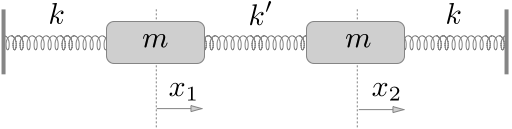
\includegraphics[width=0.5\textwidth]{coupled-oscillators.png}}
\end{center}
\[
F_1=-kx_1+k'(x_2-x_1),\quad F_2=-kx_2-k'(x_2-x_1).
\]
Les equacions del moviment són
\[
\begin{cases}
m\ddot x_1+(k+k')x_1-k'x_2=0,\\
m\ddot x_2+(k+k')x_2-k'x_1=0.\\
\end{cases}
\]
Les solucions generals,
\[
x_1=B_1e^{\lambda t},\quad x_2=B_2e^{\lambda t},
\]
i suposarem $\lambda=i\omega$. Substituint a les equacions, passen coses, estan a la llibreta. El fet és que $B_1$ i $B_2$ són diferents de zero sii
\[
\omega^2=\dfrac{k}{m}\text{ o,}\quad\omega^2=\dfrac{k+2k'}{m},
\]
les anomenades \textit{freqüències normals}.
\begin{itemize}
	\item Si $\omega^2=\dfrac{k}{m}$, aleshores $\boxed{B_1=B_2}$ i $\boxed{x_1=x_2}$. (\textit{Oscil·lacions en fase})
	\item Si, pel contrari, $\omega^2=\dfrac{k+2k'}{m}$, aleshores $\boxed{B_1=-B_2}$ i $\boxed{x_1=-x_2}$. (\textit{Oscil·lacions en oposició de fase})
\end{itemize}
La solució general serà
\[
\begin{pmatrix}x_1\\ x_2\end{pmatrix}=\begin{pmatrix}1\\ 1\end{pmatrix}B_1\cos(\omega_1t+\delta)+\begin{pmatrix}1\\ -1\end{pmatrix}B_2\cos(\omega_2t+\delta).
\]
Fent un canvi de coordenades, $\eta_1=x_1-x_2,\ \eta_2=x_1+x_2$ (els \textit{modes normals}), passen coses i
\[
\begin{pmatrix}\eta_1\\ \eta_2\end{pmatrix}=\begin{pmatrix}2B_2\cos(\omega_2t+\delta)\\ 2B_1\cos(\omega_1t+\delta)\end{pmatrix},\quad\begin{pmatrix}\omega_1\\ \omega_2\end{pmatrix}=\begin{pmatrix}\sqrt{\dfrac{k}{m}}\\ \sqrt{\dfrac{k+2k'}{m}}\end{pmatrix}.
\]
\section{Ones.}
Passen coses. Amb una corda discreta. Llibreta. Algun dia les apuntaré. La qüestió és que l'\textcolor{red}{\textit{equació d'ones}} és
\[
\boxed{
	\dfrac{\partial^2q}{\partial t^2}=\dfrac{T}{\rho}\dfrac{\partial^2q}{\partial x^2}=v^2\dfrac{\partial^2q}{\partial x^2}.
}
\]
\textcolor{red}{Solucions de l'equació d'ones:} qualsevol funció de la forma $q(x-vt)$ o $q(x+vt)$.
\subsection{Ones harmòniques.}
\[
f(x,t)=A\sin(kx-\omega t)=A\sin(k(x-vt)),\quad v=\dfrac{\omega}{k},T=\dfrac{2\pi}{\omega}=\dfrac{2\pi}{vk},\lambda=\dfrac{2\pi}{k}.
\]
\subsection{Equacions de Maxwell en absència de càrregues i corrents.}
\textit{"Otro día, vale?"}
%\chapter{Equacions diferencials: solucions generals}
\printindex


\end{document}
